\documentclass[12pt,a4paper]{article}
\title{%
  Øving 1 \\
  \large IELET1001 - Elektroteknikk \\
  }
\author{Gunnar Myhre, BIELEKTRO}

\usepackage{graphicx}
\usepackage[utf8]{inputenc}
\usepackage[norsk]{babel}
\usepackage{pgfplots}
\graphicspath{ {./images} }

\setlength\parindent{0pt}

\begin{document}
  \maketitle
  
  \section{Oppgåve 1}
    \subsection{a)}
      Elektrisk spenning $\rightarrow$ voltage (v, u)\\
      Effekt $\rightarrow$ power (P) \\
      Energi $\rightarrow$ energy (E, w)\\
      Straum $\rightarrow$ current (I) \\
      Ladning $\rightarrow$ charge (Q) \\
      Motstand $\rightarrow$ resistance (R) \\

    \subsection{b)}
      Spenning $\rightarrow$ Volt \\
      Energi $\rightarrow$ Joule (wattsekunder) \\
      Elektrisk straum $\rightarrow$ Ampere (ladningsendring over tid) \\
      Ladning $\rightarrow$ Coloumb (amperesekunder) \\

    \subsection{c)}
      \textit{Jord} er eit felles referansepunkt for 0V i ein krets. Alle andre spenninger
      i kretsen vert målt relativt til denne spenninga. \\
      To noder A og B kan ha forskjellig elektrisk potensial, og differansen mellom dei
      definerer den elektriske spenninga.

    \subsection{d)}
      Spenningen mellom node A og B vil være -24 V.

    \subsection{e)}
      Passiv Forteiknskonvensjon (PSC) hjelper oss å avgjere om eit kretselement forbruker
      eller leverer effekt til kretsen. \\
      Dersom vi definerer straumretninga inn mot positiv side av eit kretselement vil
      \begin{itemize}
        \item $vi>0$: forbruker effekt
        \item $vi<0$: leverer effekt
      \end{itemize}
  
  \section{Oppgåve 2}
    \subsection{a)}
      Elementærladninga er definert som: 
      \begin{equation}
        e = 1,602176\cdot10^{-19}C
      \end{equation}
      det går derfor
      \begin{equation}
        \frac{10C}{1,602176\cdot10^{-19}C}=6,2415\cdot10^{19}
      \end{equation}
      ladningar gjennom tverrsnittet

    \subsection{b)}
      Straumen er då på
      \begin{equation}
        \frac{10C}{20s}=0,5A
      \end{equation}

    \subsection{c)}
      \begin{equation}
        P = vi
      \end{equation}
      \begin{equation}
        i = \frac{dQ}{dt}
      \end{equation}
      \begin{equation}
        P = \frac{J}{s}
      \end{equation}
      \begin{equation}
        E = 48V\cdot9C=432J
      \end{equation}
      dersom eg antar at det er mogleg å stryke $s$ mot $dt$. Om ikkje er nok svaret
      uvisst sidan vi ikkje veit kor lang tid operasjonen tar.

    \subsection{d)}
      \begin{equation}
        i = \frac{dQ}{dt} = \frac{9C}{0,6s}=15A
      \end{equation}
      \begin{equation}
        P = \frac{J}{s} = \frac{432J}{0.6s}=720W
      \end{equation}
      \begin{equation}
        P= vi = v\frac{dQ}{dt} = 48V\frac{9C}{0,6s}=720W
      \end{equation}

  \section{Oppgåve 3}
    Sidan vi veit at
    \begin{equation}
      i = \frac{dQ}{dt}
    \end{equation}
    ser vi at straumen vil vere $10A$ i $t=0s$, $-40A$ i $t=2s$, $-5A$ i $t=3s$ og
    $50A$ i $t=5s$. \\ \\
    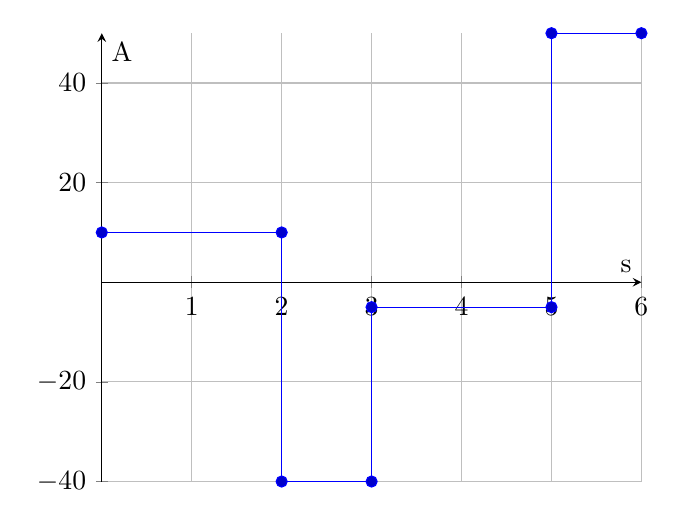
\begin{tikzpicture}
      \begin{axis}[axis lines=middle,grid=both,xlabel=s,ylabel=A]
        \addplot coordinates{
          (0,10) (2,10)
          (2,-40) (3,-40)
          (3,-5) (5,-5)
          (5,50) (6,50)};
      \end{axis}
    \end{tikzpicture}

  \newpage
  
  \section{Oppgåve 4}
    \begin{equation}
      P = vi
    \end{equation}
    \begin{itemize}
      \item $P_{1} = -15W$: leverandør
      \item $P_{2} = 5W$: forbrukar
      \item $P_{3} = 20W$: forbrukar
      \item $P_{4} = 10W$: forbrukar
      \item $P_{5} = -60W$: leverandør
      \item $P_{6} = 40W$: forbrukar
    \end{itemize}
    $-15W + 5W + 20W +10W - 60W + 40W = 0W$ \\
    Effektbalansen er overholdt.
  
  \section{Oppgåve 5}
    Ladninga som går inn i elementet er gitt ved
    \begin{equation}
      Q=i\cdot t = (10mA \cdot 10s) + \frac{(10mA \cdot 10s)}{2} = 0,15C
    \end{equation}
    sidan arealet under $i(t)$ først er ein firkant og så ein trikant.

  \section{Oppgåve 6}
    \begin{equation}
      P = \frac{J}{s} = 20W
    \end{equation}
    \begin{equation}
      i=\frac{P}{v}=1,666A
    \end{equation}
    \begin{equation}
      Q = i\cdot t = 1,666A \cdot 5s = 8,33C
    \end{equation}

  \newpage

  \section{Oppgåve 7}
    Kirchhoffs spenningslov
    \begin{equation}
      0 = 8V + 2V_{x} -V_{x}  \Rightarrow V_{x}=-8V
    \end{equation}
    \begin{equation}
      P = vi \Rightarrow P = -8V\cdot 2A = -16W 
    \end{equation}
    Sidan $P < 0$ er kretselement 2 ein leverandør.

  \section{Oppgåve 8}
    \subsection{a)}
      $v=-6V$

    \subsection{b)}
      $-9V+6V=-3V$

    \subsection{c)}
      $9V+6V=15V$

    \subsection{d)}
      $-5V+9V-3V=1V$
  
  \newpage

  \section{Oppgåve 9}
    \subsection{a)}
      Sidan lyspæra forbruker straum må straumretninga vere inn på positiv
      side av $V_{lyspære}$, som angitt på teikninga. \\ \\
      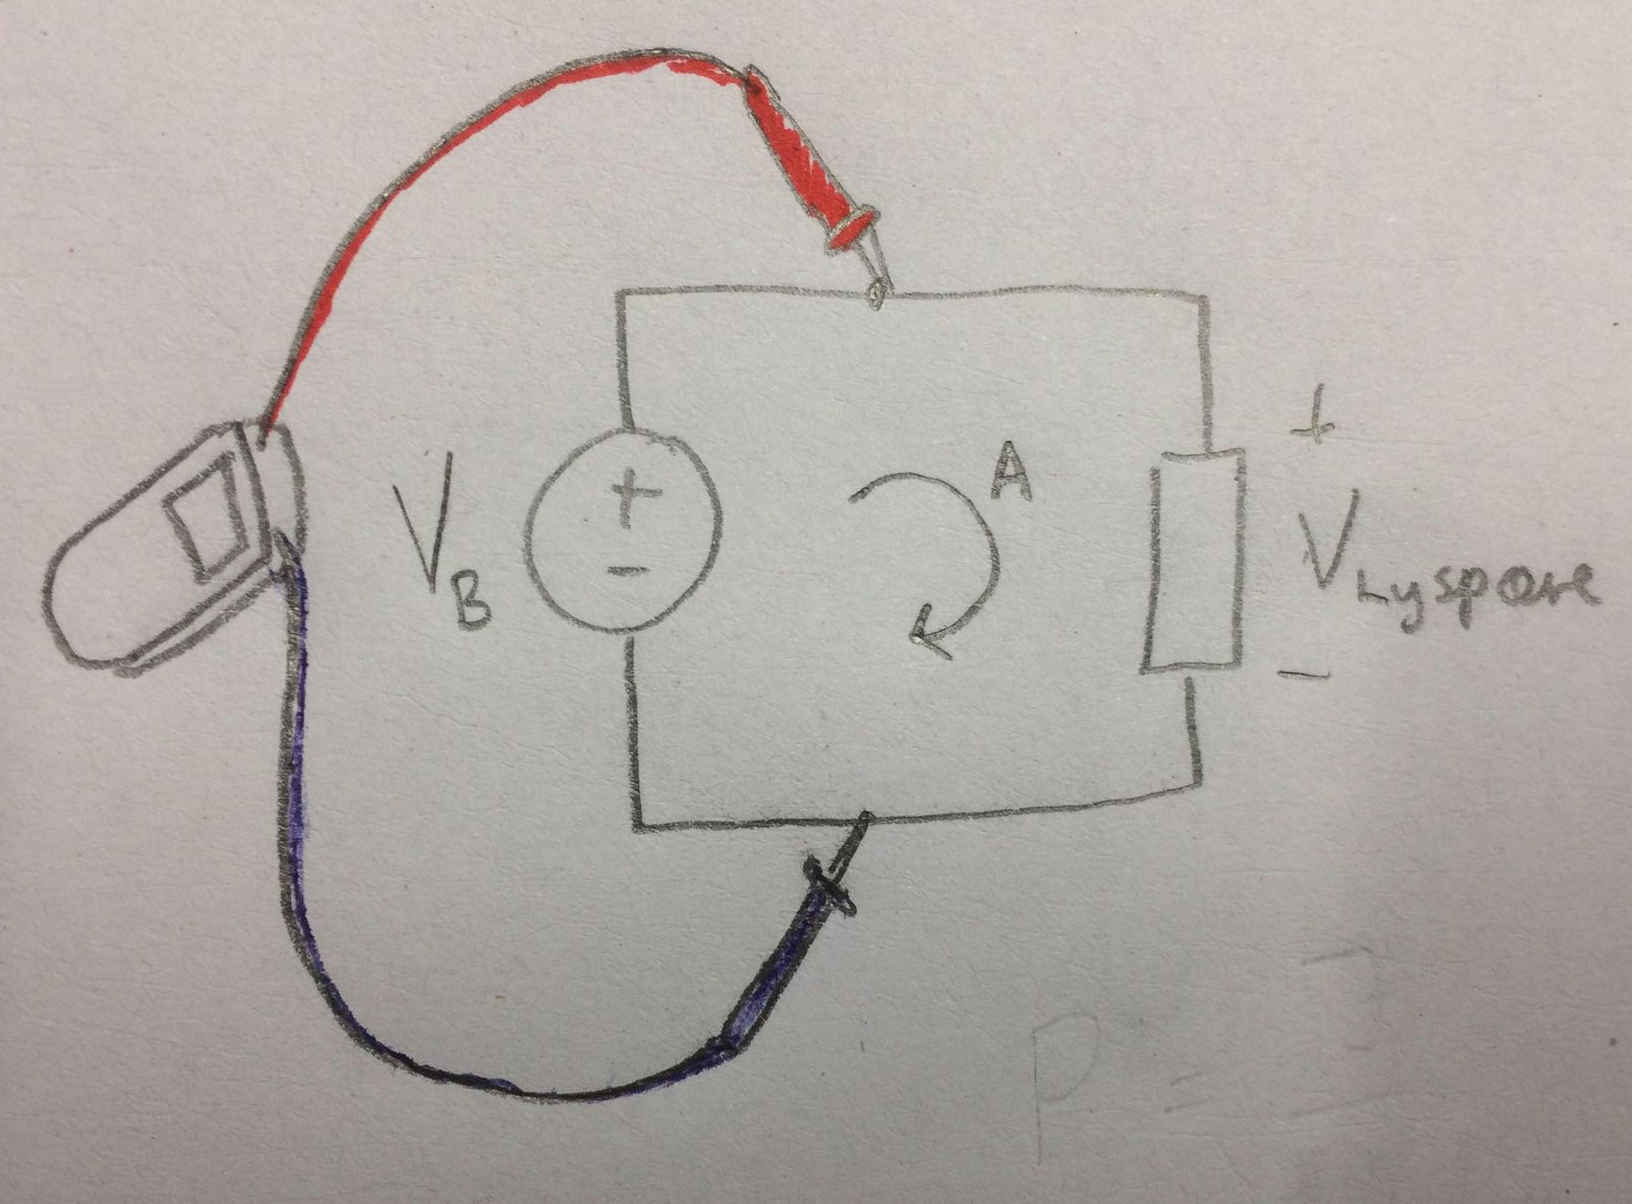
\includegraphics[width=\textwidth]{01_9_a.png}

    \subsection{b)}
      Fordi då slutter vi kretsen med kun amperemeteret som last.
      Amperemeteret har låg indre motstand sidan det egentlig
      skal koblast i serie med kretsen for å måle straum.
      Derfor vil amperemeteret bli skada.
      
\end{document}
